\documentclass{article} 
\usepackage{graphicx}
\usepackage{epstopdf}



\setlength\parindent{0pt}
\begin{document}

\begin{titlepage}
\title{System Description and Modeling of a Self-Balancing Unicycle Robot}
\author{Kevin Collins \\ Rose-Hulman Institute of Technology \\Designed for National Instruments}
\date{May 12, 2013}
\end{titlepage}

\maketitle
\newpage

\section{Introduction}
The purpose of this document is to provide a detailed explanation as to the derivation of the system model used for the self-balancing unicycle developed by Rose-Hulman's Robotics Senior Design Team G for the client, National Instruments.

\section{System Description}
The Robot is composed of a chassis made of 40mm T-slotted aluminum extrusion.  This type of frame works very well for our robot due to its modular nature.  This means, however, that many of the parameters described in this document are non-static, in that it is very possible that they have changed.  All of the calculations are as modular as possible so that any changes can be easily reflected in new calculations.  


\begin{figure}[h]
\centering
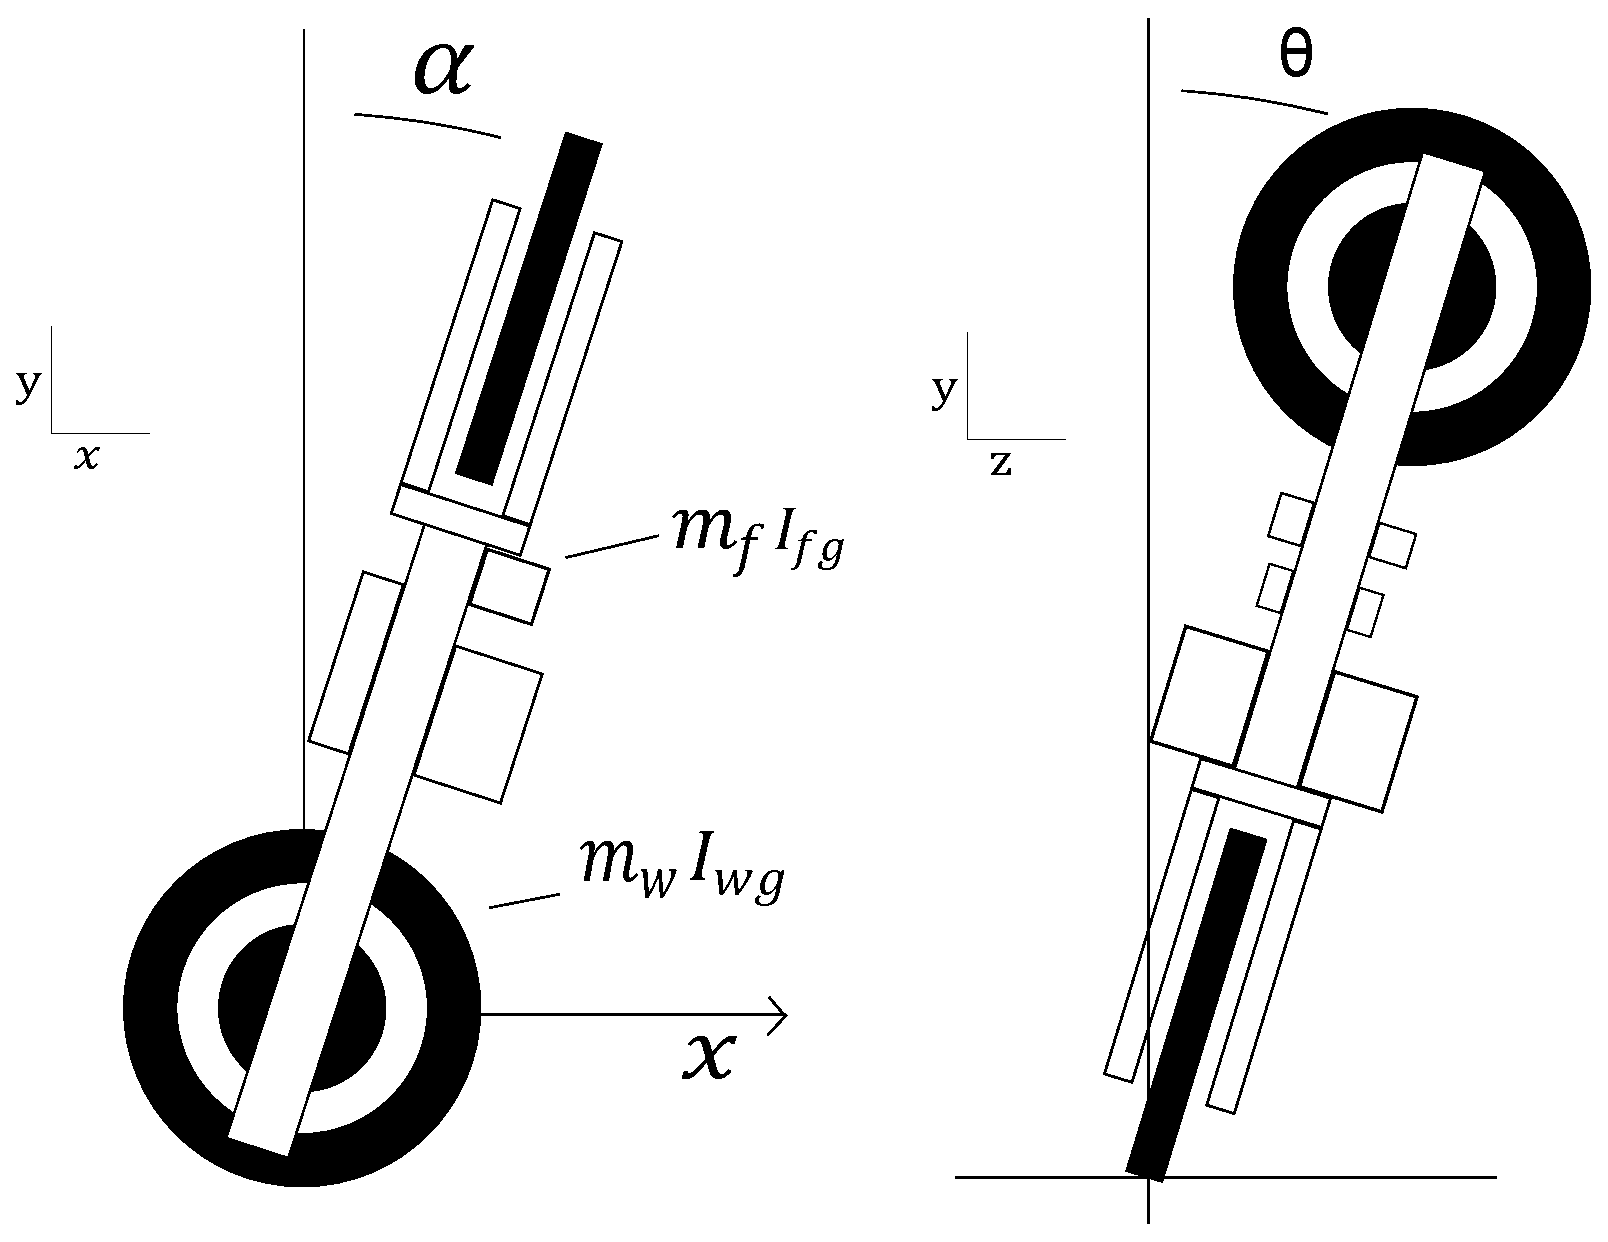
\includegraphics[scale=0.4]{systemDescriptioinDiagram}
\end{figure}

Our robot must balance in two directions: about the z axis in the x-y plane, and about the x axis about the z-y plane.    In both cases, the offset angle is measured from the inertial measurement unit located directly below the top wheel.  In the first dimension (the x-y plane) the robot corrects itself by applying a torque to the lower wheel.  In the second dimension (the z-y plane) the robot corrects itself by applying a torque to the upper wheel.

\section{First Dimension}
We start by looking at the general form of the Lagrangian equation.  The Lagrangian is used in this application because of its modular nature compared to the conservation principle approach.  If something with the model changes, the overall model can be easily updated.




\begin{equation}
 L = T - V 
 \end{equation}
 
 In the Lagrangian, T is the kinetic energy associated with the system. The kinetic energy elements of our system include the rotational energy associated with the wheel spinning, the rotational energy associated with the frame spinning about the wheel, the translational energy associated with the wheel moving in the x direction, and the translational energy with the frame moving in the x direction relative to the movement of the wheel.  These terms are shown below. \\
 
Translational energy, Wheel:
$\frac{1}{2} (m_{w} \dot{x}^2)$ \\

Translational energy, Frame: $\frac{1}{2} m_{f} (\dot{x}^2 + 2 \dot{x} r_{f} \dot{\alpha} \cos(\alpha)   + r_{f}^2 \dot{\alpha}^2)
$ \\

Rotational energy, Wheel:
$
\frac{1}{2} \left(   \frac{I_{wg} \dot{x}^2}     {r_{w}^2  } \right)
$ \\

Rotational energy, Frame:
$
\frac{1}{2} (I_{fg} \dot{\alpha}^2 )
$ \\ \\

The resulting expression for T is thus:
\begin{equation}
T = \frac{1}{2} (m_{w} \dot{x}^2) + \frac{1}{2} m_{f} (\dot{x}^2 + 2 \dot{x} r_{f} \dot{\alpha} \cos(\alpha)   + r_{f}^2 \dot{\alpha}^2)  + \frac{1}{2} \left(   \frac{I_{wg} \dot{x}^2}     {r_{w}^2  } \right) + \frac{1}{2} (I_{fg} \dot{\alpha}^2 )
\end{equation}

The V term in the Lagrangian equation is the potential energy of the system.  In this case, this is simply the weight of the frame.

\begin{equation}
V = m_{f} g r_{f} \cos(\alpha)
\end{equation}

Combining the two terms to form the Lagrangian results in:

 \begin{equation}
 L = \frac{1}{2} (m_{w} \dot{x}^2) + \frac{1}{2} m_{f} (\dot{x}^2 + 2 \dot{x} r_{f} \dot{\alpha} \cos(\alpha)   + r_{f}^2 \dot{\alpha}^2)  + \frac{1}{2} \left(   \frac{I_{wg} \dot{x}^2}     {r_{w}^2  } \right) + \frac{1}{2} (I_{fg} \dot{\alpha}^2 ) - m_{f} g r_{f} \cos(\alpha)
 \end{equation} \\

The next step is to take the following derivatives and relate them to the virtual work of the system, in this case $\tau$.

\begin{equation}
 \frac{d}{dt} \left( \frac{\partial L}{\partial \dot{\alpha}} \right) - \left( \frac{\partial L}{\partial \alpha} \right) = \tau 
 \end{equation}
 
 The resulting derivative and its expanded form are shown below:

\begin{equation}
 \left[ m_{f} r_{f}  ( \ddot{x} \cos(\alpha) - \dot{\alpha} \sin(\alpha) \dot{x}) + m_{f} r_{f}^2 \ddot{\alpha} + I_{fg} \ddot{\alpha} \right] - m_{f} \dot{x} r_{f} \dot{\alpha} \cos(\alpha) = \tau
 \end{equation}
\begin{equation}
 \ddot{x} m_{f} r_{f} \cos(\alpha) - m_{f} r_{f} \dot{\alpha} \sin(\alpha) \dot{x} + m_{f} r_{f}^2 \ddot{\alpha} + I_{fg} \ddot{\alpha} - m_{f} \dot{x} r_{f} \dot{\alpha} \cos(\alpha) = \tau       
\end{equation}\\

This model is then put into state-space form, the state variables being:

\begin{eqnarray}
z1 &=& x \nonumber \\
z2 &=& \dot{x} \nonumber \\
z3 &=& \alpha \nonumber \\
z4 &=& \dot{\alpha} \nonumber \\
\end{eqnarray} \nonumber

The state model is then as follows:
\begin{eqnarray}
\dot{z_{1}} &=& z_{2} \nonumber \\
\dot{z_{2}} &=& \frac{\tau + m_{f} z_{2} r_{f} z_{4}  \cos(z_{3}) + m_{f} r_{f} z_{4} \sin(z_{3}) z_{2}}{m_{f} r_{f} \cos(z_{3})} \nonumber \\
\dot{z_{3}} &=& z_{4} \nonumber \\
\dot{z_{4}} &=& \frac{\tau + m_{f} z_{2} r_{f} z_{4} \cos(z_{3}) + m_{f} r_{f} z_{4} sin(z_{3}) z_{2}}{m_{f} r_{f}^2 + I_{fg}} \nonumber \\
\end{eqnarray}

\newpage

 
\section{Second Dimension}
The second dimension is calculated in a similar manner as the first.  This time, T is computed from the rotation energy of the top wheel, the translational energy of the top wheel, the rotational energy of the frame, and the translational energy of the frame. 
 
\begin{equation}
T = \frac{1}{2} m_{w} \dot{x}^2 + \frac{1}{2} I_{f} \dot{\theta}^2 + \tau \theta + \frac{1}{2} m_{f} r_{f}^2 \dot{\theta}^2
\end{equation}

V is then the gravitational potential energy of the frame, and the gravitational potential energy of the wheel.

\begin{equation}
V = m_{f} g L_{1} \cos(\theta) + m_{w} g (L_{1} + L_{2}) \cos(\theta)
\end{equation}

The Lagrangian is:
\begin{equation}
L = T - V
\end{equation}

Which, when evaluated with the above equations, results in the following:
\begin{equation}
L = \frac{1}{2} m_{w} \dot{x}^2 + \frac{1}{2} I_{f} \dot{\theta}^2 + \tau \theta + \frac{1}{2} m_{f} r_{f}^2 \dot{\theta}^2 - m_{f} g L_{1} \cos(\theta) - m_{w} g (L_{1} + L_{2}) \cos(\theta)
\end{equation}

Taking the partial derivatives results in the following equations:

\begin{equation}
\frac{\partial{L}}{\partial{{\theta}}} =  m_{f} g L_{1} \cos(\theta)  m_{w} g (L_{1} + L_{2}) \cos(\theta) + \tau
\end{equation}

\begin{equation}
\frac{\partial{L}}{\partial{\dot{\theta}}} = I_{f} \dot{\theta} + m_{f} r_{f}^2 \dot{\theta}
\end{equation}

\begin{equation}
\frac{d}{dt} \left(\frac{\partial{L}}{\partial{\dot{\theta}}}\right) = I_{f} \ddot{\theta} + m_{f} r_{f}^2 \ddot{\theta}
\end{equation}

\begin{equation}
\frac{d}{dt} \left(\frac{\partial{L}}{\partial{\dot{\theta}}}\right) - \frac{\partial{L}}{\partial{\dot{\theta}}} = I_{f} \ddot{\theta} + m_{f} r_{f}^2 \ddot{\theta} -  m_{f} g L_{1} \cos(\theta)  m_{w} g (L_{1} + L_{2}) \cos(\theta) + \tau
\end{equation}

which is equal to the virtual work of the system.  This equation can then be put into state space form as shown in the first dimension.



\newpage
\section{Moment of Inertia Calculations}
For our system, the moment of inertia was was calculated by combining the moment of inertia of the following elements:
\begin{itemize}
\item Top Components - top wheel, top fork, top junction
\item Middle Components - IMU, e-stop power1, power2, dc-dc converter, relay, breaker, controller, battery1, battery2, cRIO, center column
\item Lower Components - bottom wheel, bottom fork1, bottom fork2, bottom junction \\
\end{itemize} 

\begin{figure}[h]
\centering
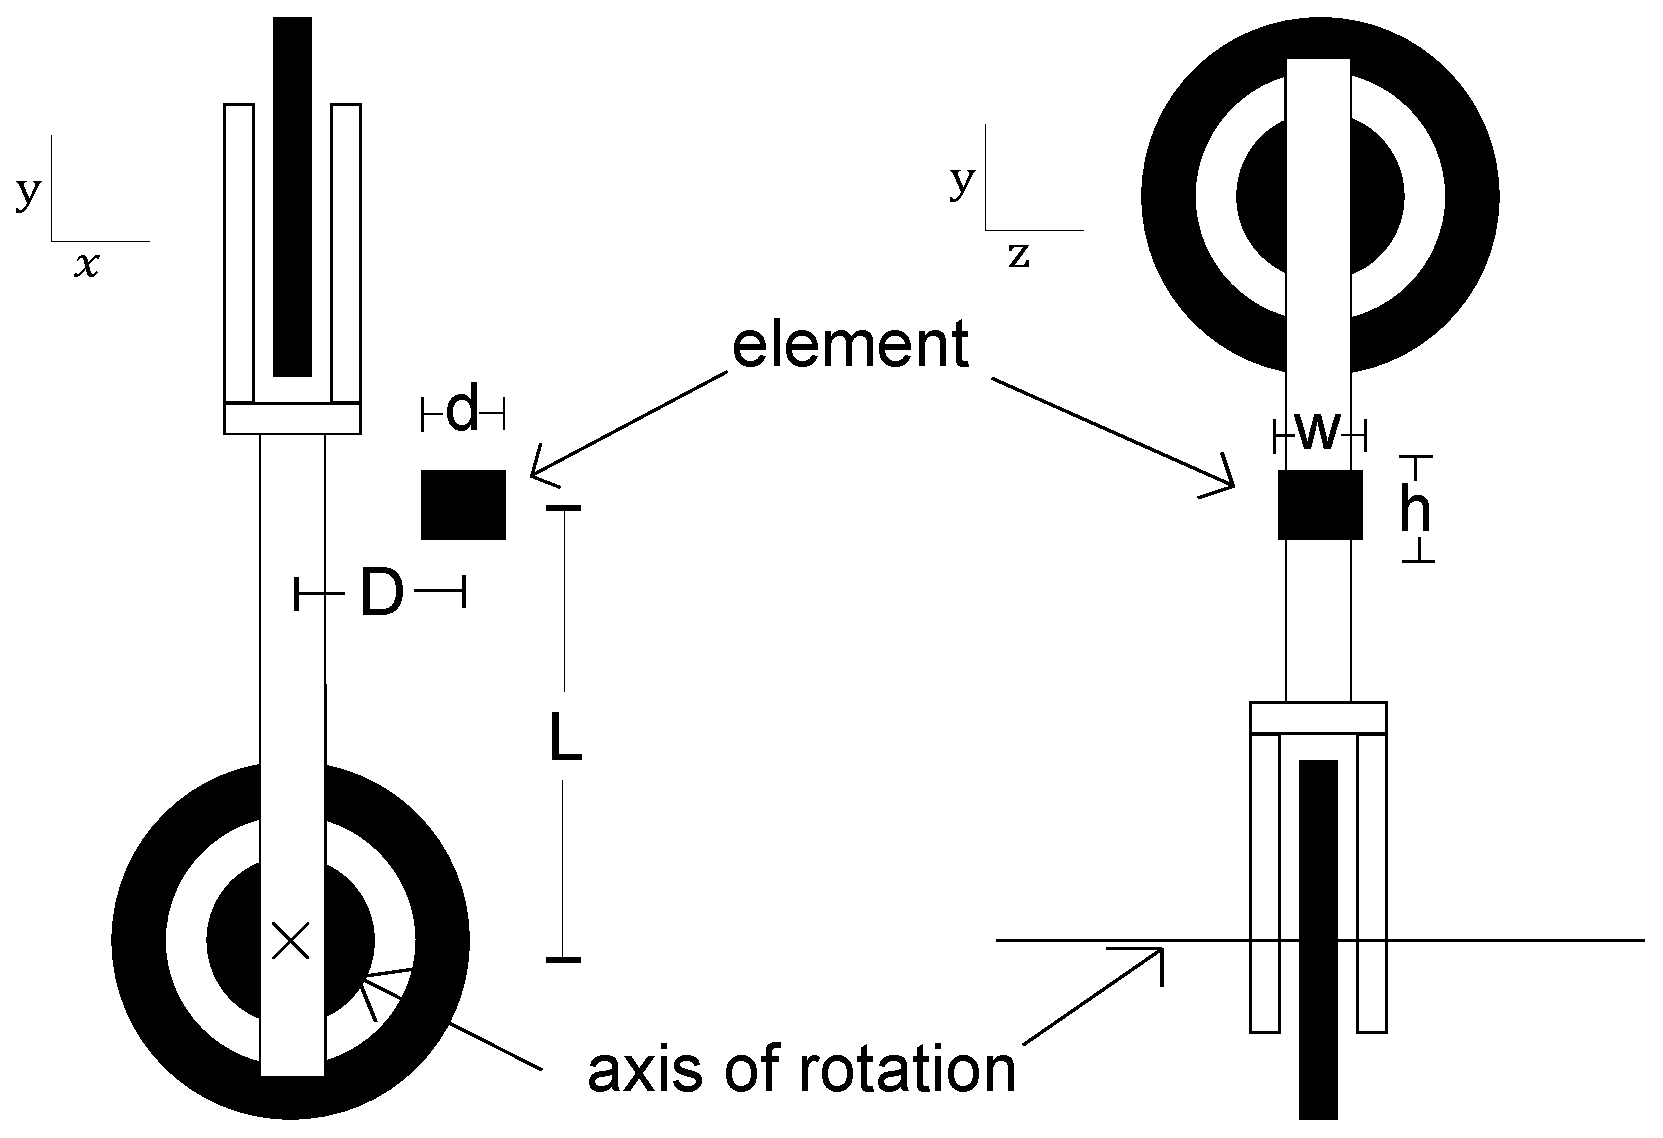
\includegraphics[scale=0.4]{momentOfInertiaDiagram}\\
\end{figure}

The equations for a moment of inertia of an object in 3d about an axis are represented by the following equations:
\begin{eqnarray}
I_{h} &=& \frac{1}{12} m(w^2 + d^2) \nonumber \\
I_{w} &=& \frac{1}{12} m(h^2 + d^2) \nonumber \\
I_{d} &=& \frac{1}{12} m(h^2 + w^2) \nonumber \\
\end{eqnarray}

In the system described in section 1, the first dimension has a rotation about the d axis.  The equations above are valid if the elements are rotated about an axis that runs through the center of mass of the element.  The axis of rotation for most of our elements do not run through the center of mass, so to calculate this value, we use the parallel axis theorem.  The parallel axis theorem can determine the moment of inertia about any axis given the moment of inertia about a parallel axis that passes through the center of gravity of the element, and the perpendicular distance between the two axes (r).  

\begin{equation}
I_{z} = I_cm + mr^2
\end{equation}


 
In the 3d case, $r^2$ has two vector components to it, resulting in an absolute distance from the axis of rotation.  Many of our components are centered directly above the axis of rotation, so the third dimension is 0, but this is still accounted for in our calculation.\\

The rotation axis of the first dimension is about the axle of the lower motor.  The rotation axis of the 2nd dimension is about the axis running along the length of the wheel where it contacts the ground.\\

All of the components on our robot were modeled as either rectangular prisms or solid cylinders.\\

For a solid rectangular prism, the equation for the moment of inertia about a given axis with 


\newpage
\section{Suggestions for Improvement}
As stated in the previous section, all of the components on our robot were modeled as either rectangular prisms or solid cylinders.  This is an extreme simplification, especially in the case of the motors.  If more work was to be done in modeling the system, I would suggest that a more accurate model of the wheels be determined first.\\

As far as the second dimension goes, these equations were not verified the same way that the first dimension was.  The equations of motion were derived the same way they were for the first dimension, but they should be verified before deployed in a controller.



\end{document}